\documentclass[11pt,a4paper]{article}

\usepackage[utf8]{inputenc}
\usepackage[T1]{fontenc}
\usepackage{lmodern}
\usepackage[margin=2.3cm]{geometry}
\usepackage{amsmath,amssymb,bm}
\usepackage{graphicx}
\usepackage{booktabs}
\usepackage{caption}
\usepackage{subcaption}
\usepackage{float}
\usepackage{xcolor}
\usepackage{microtype}
\usepackage{parskip}
\usepackage{enumitem}
\usepackage[hidelinks]{hyperref}
\setlength{\emergencystretch}{1.5em}

\captionsetup{font=small,labelfont=bf,skip=4pt}
\graphicspath{{figures/}}

\newcommand{\R}{\mathbb{R}}
\newcommand{\argmin}{\operatorname*{arg\,min}}
\newcommand{\T}{\top}
\newcommand{\diag}{\operatorname{diag}}
\newcommand{\vecop}{\operatorname{vec}}

\title{\vspace{-1.4cm}
\textbf{Laboratory 2:}\\[2pt]
\textbf{Basic Optimization and\\[2pt] Introduction to Inverse Problems}\\[6pt]
\large Written Solution: Calculations, Explanations, and Answers}
\author{HDSP Research Group\\
School of Systems and Computer Engineering\\
Universidad Industrial de Santander}
\date{Trial Period --- 2026}

\begin{document}
\maketitle

\vspace{-0.5cm}
\noindent\rule{\textwidth}{0.4pt}\par
\small
This document is the written solution of Laboratory~2. All numerical values, figures, and
conclusions were produced by the accompanying notebook \texttt{lab2.ipynb}; the figures are
reproduced directly from its outputs. Section~\ref{sec:opt} solves the calculus exercises,
Section~\ref{sec:ls} the least-squares and pseudoinverse experiment, Section~\ref{sec:inv} the
deconvolution problem, Section~\ref{sec:ista} the regularized reconstruction with a sparse
wavelet prior, and Section~\ref{sec:priors} a comparison of that prior with Tikhonov smoothness
and total variation. The theoretical background follows the workshop notes~\cite{heckel2024}.

\normalsize
\noindent\rule{\textwidth}{0.4pt}\par

%=====================================================================
\section{Optimization in one and two dimensions}\label{sec:opt}

\subsection{Notation and interpretation}

An optimization problem is written as $\min_{x\in\mathcal{D}} f(x)$. In plain words, among all
admissible choices $x$ we keep the one that makes $f$ as small as possible. The \emph{decision
variable} $x$ is what we are free to choose (a scalar, a vector, a signal, or an image stored as a
long vector); the \emph{objective} $f(x)$ assigns a single number (cost, error, energy) to each
candidate, and smaller values are better. A maximization is handled by minimizing $-f$, e.g.\
maximizing profit is the same as minimizing negative profit. A point $x^\star$ is a
\emph{global} minimizer if $f(x^\star)\le f(x)$ for every admissible $x$, and a \emph{local}
minimizer if the inequality holds in a neighborhood of $x^\star$. Practical examples: in delivery
planning $x$ is the route and $f$ is fuel, driver time, and delay penalties; in linear regression
$x$ is the coefficient vector and $f$ is the prediction error; in image deblurring $x$ is the
unknown clean image and $f$ combines data mismatch with a regularizer; in portfolio design $x$ is
the amount invested in each asset and $f$ balances risk and return. In this report $x$ is a scalar
(Section~\ref{sec:opt}), a pair $(x,y)$, a coefficient vector in $\R^n$ (Section~\ref{sec:ls}), or
an image vector in $\R^N$ (Sections~\ref{sec:inv}--\ref{sec:ista}). For a differentiable
objective, candidates are located by setting the gradient to zero and are classified with the
second-order information (second derivative in 1D, Hessian in 2D).

\subsection{Exercise 1 (1D): minimize \texorpdfstring{$f(x)=x^4-4x^2+x$}{f(x) = x4 - 4x2 + x}}

The derivatives are
\begin{equation}
f'(x)=4x^3-8x+1,
\qquad
f''(x)=12x^2-8 .
\label{eq:d1}
\end{equation}
Stationary points satisfy $f'(x)=0$, that is,
\begin{equation}
4x^3-8x+1=0
\quad\Longleftrightarrow\quad
x^3-2x+\tfrac14=0 .
\label{eq:cubic}
\end{equation}
For a depressed cubic $x^3+px+q$ with $p=-2$ and $q=\tfrac14$, the discriminant is
\begin{equation}
\Delta=\left(\frac{q}{2}\right)^2+\left(\frac{p}{3}\right)^3
=\frac{1}{64}-\frac{8}{27}
=-\frac{485}{1728}\approx -0.2807<0 .
\label{eq:disc}
\end{equation}
A negative discriminant means that the cubic has three distinct real roots. They are computed
numerically with \texttt{np.roots} and listed in Table~\ref{tab:1d}; at every root the residual
$|f'(x^\star)|$ is below $2\times10^{-15}$, confirming stationarity.

\begin{table}[H]
\centering
\small
\begin{tabular}{cccc}
\toprule
$x^\star$ & $f(x^\star)$ & $f''(x^\star)$ & Classification (second-derivative test)\\
\midrule
$-1.472998$ & $-5.444192$ & $18.036663$ & local minimum\\
$0.126000$  & $0.062748$  & $-7.809487$ & local maximum\\
$1.346997$  & $-2.618556$ & $13.772824$ & local minimum\\
\bottomrule
\end{tabular}
\caption{Critical points of $f(x)=x^4-4x^2+x$ and their classification.}
\label{tab:1d}
\end{table}

Since $f''>0$ at $x\approx-1.4730$ and $x\approx1.3470$, both are local minima, whereas
$f''<0$ at $x\approx0.1260$, which is a local maximum. The quartic is coercive
($f(x)\to+\infty$ as $|x|\to\infty$), so a global minimum exists and must be one of the local
minima. Comparing their values,
\[
f(-1.472998)=-5.444192 \;<\; f(1.346997)=-2.618556 .
\]

\paragraph{Answer.}
The critical points are $x_1^\star\approx-1.4730$ (local minimum),
$x_2^\star\approx0.1260$ (local maximum), and $x_3^\star\approx1.3470$ (local minimum). The
global minimum over $\R$ is
\[
x^\star\approx-1.4730,
\qquad f(x^\star)\approx-5.4442 .
\]
Figure~\ref{fig:1d} shows the graph with the three stationary points; the global minimum is
marked in red and the dotted line is its function value.

\begin{figure}[htbp]
\centering
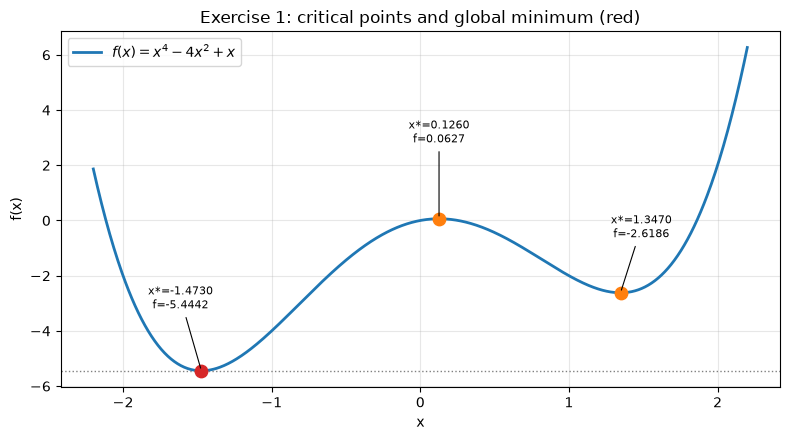
\includegraphics[width=\textwidth]{fig01_1d.png}
\caption{Exercise 1: graph of $f(x)=x^4-4x^2+x$ with the three critical points (the global
minimum in red). The dotted horizontal line marks $f(x^\star)\approx-5.4442$.}
\label{fig:1d}
\end{figure}

\subsection{Exercise 2 (2D): minimize \texorpdfstring{$f(x,y)=x^2+xy+y^2-4x-6y$}{f(x,y) = x2 + xy + y2 - 4x - 6y}}

The gradient is
\begin{equation}
\nabla f(x,y)=
\begin{bmatrix}
2x+y-4\\[2pt]
x+2y-6
\end{bmatrix}.
\label{eq:grad2d}
\end{equation}
Setting $\nabla f=0$ gives the linear system
\[
\begin{cases}
2x+y=4,\\
x+2y=6.
\end{cases}
\]
From the first equation $y=4-2x$. Substituting into the second,
\[
x+2(4-2x)=6 \;\Longrightarrow\; -3x=-2 \;\Longrightarrow\; x^\star=\frac23,
\qquad y^\star=4-2\cdot\frac23=\frac83 .
\]
The Hessian is constant:
\begin{equation}
H=\nabla^2 f(x,y)=
\begin{bmatrix}
2 & 1\\
1 & 2
\end{bmatrix},
\qquad
\det(H-\lambda I)=(2-\lambda)^2-1=0
\;\Longrightarrow\;
\lambda_1=1,\ \lambda_2=3 .
\label{eq:hess2d}
\end{equation}
Both eigenvalues are positive, so $H$ is positive definite. Equivalently,
$D=f_{xx}f_{yy}-f_{xy}^2=\det H=3>0$ and $f_{xx}=2>0$. Since $H$ is positive definite
everywhere, $f$ is strongly convex and the stationary point is the unique global minimizer.
Its value is
\begin{equation}
f\!\left(\frac23,\frac83\right)
=\frac49+\frac{16}{9}+\frac{64}{9}-\frac83-16
=\frac{28}{3}-\frac83-16
=-\frac{28}{3}\approx-9.3333 .
\label{eq:fmin2d}
\end{equation}

\paragraph{Answer.}
The unique critical point is $(x^\star,y^\star)=(2/3,\,8/3)$. The Hessian is positive definite
($\lambda_{1,2}=1,3$; $D=3>0$), hence it is a strict local minimum and, by convexity, the
\emph{global} minimum, with $f_{\min}=-28/3\approx-9.3333$. Figure~\ref{fig:2d} shows the level
curves and the surface.

\begin{figure}[htbp]
\centering
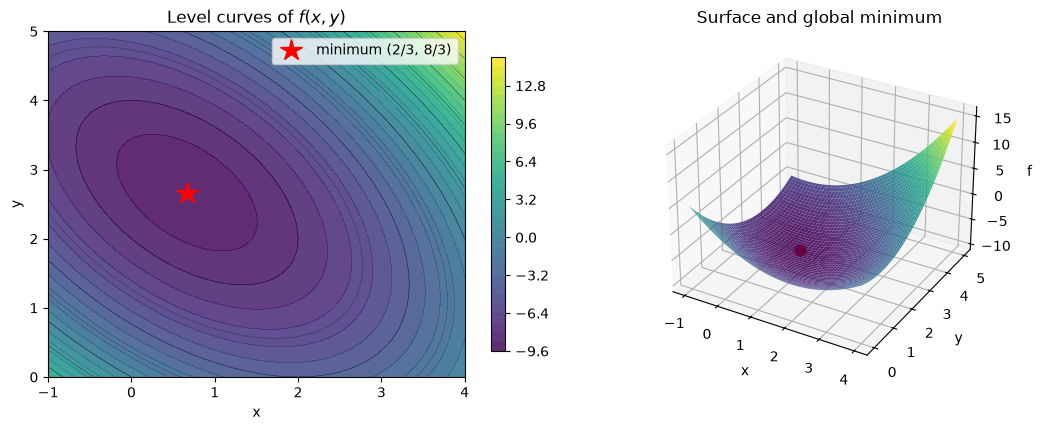
\includegraphics[width=\textwidth]{fig02_2d.png}
\caption{Exercise 2: level curves (left) and surface (right) of
$f(x,y)=x^2+xy+y^2-4x-6y$, with the global minimum at $(2/3,8/3)$.}
\label{fig:2d}
\end{figure}

\subsection{Exercise: gradient of the least-squares residual}

The Euclidean norm of $v\in\R^n$ is
\begin{equation}
\|v\|_2=\left(\sum_{i=1}^{n}v_i^2\right)^{1/2}.
\label{eq:norm}
\end{equation}
Let $B\in\R^{n\times n}$ and $h(x)=x^\T Bx=\sum_i\sum_j x_iB_{ij}x_j$. Differentiating with
respect to $x_k$,
\[
\frac{\partial h}{\partial x_k}
=\sum_{j=1}^{n}B_{kj}x_j+\sum_{i=1}^{n}x_iB_{ik}
=(Bx)_k+(B^\T x)_k ,
\]
so
\begin{equation}
\nabla_x\!\left(x^\T Bx\right)=(B+B^\T)x .
\label{eq:gradquad}
\end{equation}
For $B=A^\T A$, which is symmetric, this gives the identity
\begin{equation}
\nabla_x\|Ax\|_2^2=\nabla_x\!\left(x^\T A^\T A x\right)=2A^\T A x .
\label{eq:gradAx}
\end{equation}
For the residual, write
\[
r(x)=\|Ax-y\|_2^2=(Ax-y)^\T(Ax-y)
=x^\T A^\T A x-2\,x^\T A^\T y+y^\T y .
\]
Applying \eqref{eq:gradquad} to the first term and $\nabla_x(x^\T A^\T y)=A^\T y$ to the
second,
\begin{equation}
\nabla r(x)=2A^\T A x-2A^\T y=2A^\T(Ax-y).
\label{eq:gradres}
\end{equation}

\paragraph{Answer.}
\[
\boxed{\;\nabla_x\|Ax-y\|_2^2=2A^\T(Ax-y)\;}
\]
Consequently $\nabla_x\!\left(\tfrac12\|Ax-y\|_2^2\right)=A^\T(Ax-y)$. Setting this gradient
to zero yields the normal equations $A^\T A x=A^\T y$.

%=====================================================================
\section{Least squares and the pseudoinverse in \texorpdfstring{$\R^n$}{Rn}}\label{sec:ls}

\subsection{Normal equations and the pseudoinverse}

Given $A\in\R^{m\times n}$ and $y\in\R^m$, the least-squares problem is
\begin{equation}
\min_{x\in\R^n}\;\|Ax-y\|_2^2 .
\label{eq:ls}
\end{equation}
Because $\nabla\|Ax-y\|^2=2A^\T(Ax-y)$, stationarity gives the normal equations
\begin{equation}
A^\T A\,x^\star=A^\T y .
\label{eq:normal}
\end{equation}
If $A$ has full column rank ($m\ge n$ and $\operatorname{rank}A=n$), $A^\T A$ is invertible and
\begin{equation}
x^\star=(A^\T A)^{-1}A^\T y=A^\dagger y ,
\label{eq:fullrank}
\end{equation}
where $A^\dagger$ is the Moore--Penrose pseudoinverse.

With the singular value decomposition (SVD)
$A=U\Sigma V^\T=\sum_{i=1}^{r}\sigma_i u_i v_i^\T$, where $r=\operatorname{rank}A$, the
pseudoinverse is
\begin{equation}
A^\dagger=V\Sigma^\dagger U^\T=\sum_{i=1}^{r}\frac{1}{\sigma_i}\,v_i u_i^\T ,
\label{eq:svdpinv}
\end{equation}
and $x^\star=A^\dagger y$ is the least-squares solution of minimum norm. Two cases are relevant:
\begin{itemize}[leftmargin=1.4em,itemsep=1pt]
\item \textbf{Overdetermined ($m>n$, full column rank).} The solution is unique and given by
\eqref{eq:fullrank}. Owing to the noise, the residual $\|Ax^\star-y\|_2$ is generally nonzero.
\item \textbf{Underdetermined ($m<n$, full row rank).} The system is consistent and has
infinitely many solutions. Then $A^\dagger=A^\T(AA^\T)^{-1}$ and $x^\star$ is the solution of
smallest norm, i.e., the orthogonal projection of any solution onto the row space of $A$.
\end{itemize}

\subsection{Numerical comparison: \texttt{pinv} versus \texttt{lstsq}}

The experiment follows the notebook. For each case, $A\in\R^{m\times n}$ and
$x_{\text{true}}\in\R^n$ are drawn from $\mathcal{N}(0,1)$ with fixed seeds, and the measurements
are
\[
y=Ax_{\text{true}}+\sigma e,\qquad e\sim\mathcal{N}(0,I_m),\qquad \sigma=0.05 .
\]
The two estimates are $\hat{x}_{\text{pinv}}=\operatorname{pinv}(A)y$ and
$\hat{x}_{\text{lstsq}}=\texttt{lstsq}(A,y)$, and they are assessed with
\begin{equation}
\text{relative error}=\frac{\|\hat{x}-x_{\text{true}}\|_2}{\|x_{\text{true}}\|_2},
\qquad
\text{residual}=\|A\hat{x}-y\|_2 .
\label{eq:metrics}
\end{equation}
The dimensions are $(m,n)=(80,20)$ for the overdetermined case (seed 1) and $(m,n)=(20,80)$ for
the underdetermined case (seed 2). The results are reported in Table~\ref{tab:pinv}.

\begin{table}[H]
\centering
\small
\begin{tabular}{llcc}
\toprule
Case & Method & Relative error & Residual\\
\midrule
$m>n$ \ ($80\times20$) & \texttt{pinv}  & $4.471\times10^{-3}$ & $4.148\times10^{-1}$\\
                       & \texttt{lstsq} & $4.471\times10^{-3}$ & $4.148\times10^{-1}$\\
\addlinespace
$m<n$ \ ($20\times80$) & \texttt{pinv}  & $8.928\times10^{-1}$ & $4.759\times10^{-14}$\\
                       & \texttt{lstsq} & $8.928\times10^{-1}$ & $4.578\times10^{-14}$\\
\bottomrule
\end{tabular}
\caption{Pseudoinverse versus \texttt{lstsq}. The maximum coefficient differences between the two
methods are $1.01\times10^{-14}$ ($m>n$) and $5.46\times10^{-15}$ ($m<n$).}
\label{tab:pinv}
\end{table}

\paragraph{Overdetermined case.}
Both methods return the same vector up to roundoff ($1.01\times10^{-14}$), because they solve the
same normal equations. The residual $0.4148$ is of the expected size for Gaussian noise after
projecting onto an $(m-n)$-dimensional subspace, $\sigma\sqrt{m-n}=0.05\sqrt{60}\approx0.387$.
The coefficient error is of order $\sigma/\sqrt{m}\approx5.6\times10^{-3}$, in agreement with the
observed $4.47\times10^{-3}$: the estimate is close to $x_{\text{true}}$, but the residual cannot
be reduced to zero because of the noise. Figure~\ref{fig:bars} compares the metrics and
Figure~\ref{fig:scatter} the recovered coefficients.

\begin{figure}[htbp]
\centering
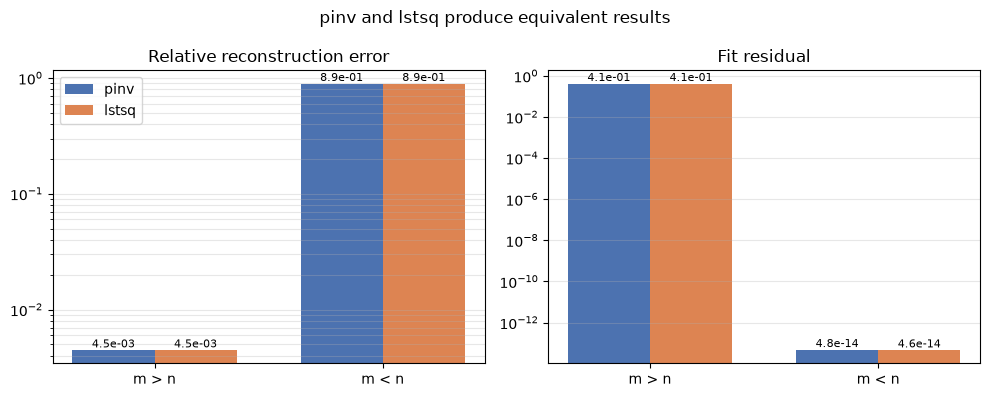
\includegraphics[width=0.98\textwidth]{fig03_pinv_bars.png}
\caption{Relative reconstruction error (left) and fit residual (right) for \texttt{pinv} and
\texttt{lstsq}. The vertical axis is logarithmic; the two methods give bars of equal height.}
\label{fig:bars}
\end{figure}

\paragraph{Underdetermined case.}
The residual is at machine precision ($\sim5\times10^{-14}$), so the measurements are fitted
exactly, but the relative coefficient error is $0.893$. This is not a numerical failure: with only
$20$ measurements for $80$ unknowns, the solution is not unique, and \texttt{pinv}/\texttt{lstsq}
return the minimum-norm solution. For a random Gaussian matrix, that solution is the projection of
$x_{\text{true}}$ onto a random $20$-dimensional row space, whose expected relative error is
\[
\sqrt{1-\frac{n}{m}}=\sqrt{1-\frac{20}{80}}=\sqrt{0.75}\approx0.866,
\]
consistent with the observed $0.893$.

\paragraph{Answer to item 4.}
In the case $m<n$ the pseudoinverse returns the \emph{minimum-norm least-squares solution}
$x^\star=A^\T(AA^\T)^{-1}y$. It reproduces the data with zero residual, but it does not recover the
true vector, since infinitely many coefficient vectors produce the same measurements. A small
residual therefore does not imply a small reconstruction error.

\begin{figure}[htbp]
\centering
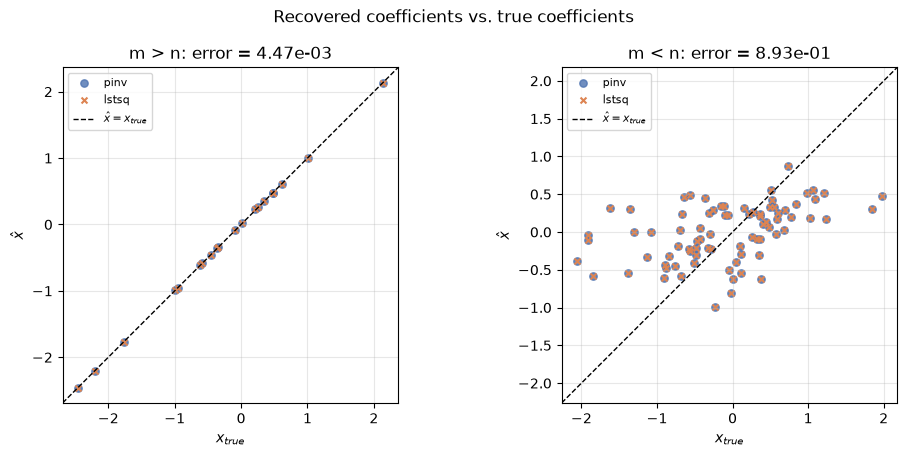
\includegraphics[width=0.92\textwidth]{fig04_coefficients.png}
\caption{Recovered coefficients $\hat{x}$ versus the true coefficients $x_{\text{true}}$. In the
overdetermined case the points lie on the diagonal; in the underdetermined case the minimum-norm
solution is far from $x_{\text{true}}$ even though the residual is essentially zero.}
\label{fig:scatter}
\end{figure}

%=====================================================================
\section{Linear inverse problems: deconvolution and instability}\label{sec:inv}

\subsection{Forward model and explicit blur operator}

A grayscale image $X\in\R^{48\times48}$ (the \texttt{camera} image, normalized to $[0,1]$) is
vectorized as $x=\vecop(X)\in\R^N$ with $N=48^2=2304$. The blur is a two-dimensional convolution
with a normalized Gaussian kernel of size $9\times9$ ($r=4$) and standard deviation
$\sigma_k=1.5$:
\begin{equation}
k[i,j]=\frac{1}{Z}\exp\!\left(-\frac{i^2+j^2}{2\sigma_k^2}\right),
\qquad -r\le i,j\le r,
\qquad
Z=\sum_{i,j}\exp\!\left(-\frac{i^2+j^2}{2\sigma_k^2}\right),
\label{eq:kernel}
\end{equation}
with symmetric (reflection) boundary conditions. The kernel sums to one,
$\sum_{i,j}k[i,j]=1$, so a constant image is preserved.

The matrix $A\in\R^{N\times N}$ is built column by column: for each pixel index $j$, a basis image
$E_j$ (zero except for a one at pixel $j$) is blurred, and the result is stored as column $j$,
\begin{equation}
A_{:,j}=\vecop\!\left(\operatorname{blur}(E_j)\right).
\label{eq:Acol}
\end{equation}
Thus $A$ represents the blur exactly, and the forward model is
\begin{equation}
y=Ax,\qquad y_\eta=Ax+e,\qquad e\sim\mathcal{N}(0,\sigma_\eta^2 I_N),
\label{eq:forward}
\end{equation}
with $\sigma_\eta=0.005$. The constructed matrix has $2304^2=5{,}308{,}416$ entries and is
symmetric: $\max|A-A^\T|=2.78\times10^{-17}$.

\subsection{Pseudoinverse reconstruction and noise amplification}

With the SVD $A=U\Sigma V^\T$, the pseudoinverse is $A^\dagger=V\Sigma^{-1}U^\T$ and the estimate
is $\hat{x}=A^\dagger y_\eta$. Since $y_\eta=Ax+e$ and $A^\dagger A=I$ (the blur matrix is
invertible), the error is
\begin{equation}
\hat{x}-x=A^\dagger e=\sum_{i=1}^{N}\frac{u_i^\T e}{\sigma_i}\,v_i ,
\qquad
\|\hat{x}-x\|_2\le\frac{1}{\sigma_{\min}}\|e\|_2 .
\label{eq:errorprop}
\end{equation}
Because $\|y\|_2\le\sigma_{\max}\|x\|_2$, the relative error satisfies
\begin{equation}
\frac{\|\hat{x}-x\|_2}{\|x\|_2}
\le \kappa(A)\,\frac{\|e\|_2}{\|y\|_2},
\qquad
\kappa(A)=\frac{\sigma_{\max}}{\sigma_{\min}} .
\label{eq:bound}
\end{equation}
This is the standard noise-amplification mechanism of ill-conditioned inverse
problems~\cite{hansen2010}. The computed condition number is $\kappa(A)=2.44\times10^{8}$, while the relative noise level is
$\|e\|_2/\|y\|_2=7.96\times10^{-3}$. The observed amplification
$\|\hat{x}_{\text{noisy}}-x\|_2/\|e\|_2=4.38\times10^{6}$ is large but below the worst-case
factor $1/\sigma_{\min}\approx2.4\times10^{8}$, because a random perturbation is not aligned with
the weakest singular direction.

\begin{table}[H]
\centering
\small
\begin{tabular}{lcc}
\toprule
Result & PSNR (dB) & SSIM\\
\midrule
Blurred measurement $y$                     & $23.49$  & $0.812$\\
Pseudoinverse, clean data                   & $187.72$ & $1.000$\\
Measurement with noise $y_\eta$             & $23.45$  & $0.804$\\
Pseudoinverse, noisy data                   & $-86.90$ & $0.000$\\
Original image plus noise $x+e$             & $45.94$  & $0.993$\\
Inverting noise added before the blur       & $45.94$  & $0.993$\\
\bottomrule
\end{tabular}
\caption{Reconstruction quality for the deconvolution experiment. PSNR uses
$\mathrm{PSNR}=10\log_{10}(1/\mathrm{MSE})$ with data range $1$; SSIM is computed with
\texttt{skimage.metrics.structural\_similarity} and \texttt{data\_range=1}.}
\label{tab:deconv}
\end{table}

The quality metrics are the mean squared error, the peak signal-to-noise ratio, and the
structural similarity index~\cite{wang2004}:
\begin{equation}
\mathrm{MSE}=\frac{1}{N}\|x-\hat{x}\|_2^2,
\qquad
\mathrm{PSNR}=10\log_{10}\!\left(\frac{1}{\mathrm{MSE}}\right)\ \text{dB},
\label{eq:psnr}
\end{equation}
\begin{equation}
\mathrm{SSIM}(X,\hat{X})=
\frac{(2\mu_X\mu_{\hat X}+c_1)(2\sigma_{X\hat X}+c_2)}
{(\mu_X^2+\mu_{\hat X}^2+c_1)(\sigma_X^2+\sigma_{\hat X}^2+c_2)},
\label{eq:ssim}
\end{equation}
computed over local windows and averaged. Larger PSNR and SSIM indicate a better reconstruction;
SSIM is closer to one when the local luminance, contrast, and structure match.

The results in Table~\ref{tab:deconv} and Figure~\ref{fig:deconv} show three regimes.
\begin{itemize}[leftmargin=1.4em,itemsep=1pt]
\item \textbf{Clean data.} The pseudoinverse recovers the image with maximum absolute error
$1.73\times10^{-9}$ and PSNR $187.72$~dB, i.e., the inversion is accurate up to roundoff
(Figure~\ref{fig:deconv}c).
\item \textbf{Noise added after the blur.} The reconstruction has PSNR $-86.90$~dB and SSIM
$0.000$: the amplified noise completely dominates the image (Figure~\ref{fig:deconv}e). The
displayed image is clipped to $[0,1]$ only for visualization; the metrics use the unclipped
values.
\item \textbf{Noise added before the blur.} Here $y'=A(x+e)$ and
$\hat{x}'=A^\dagger y'=x+e$ up to roundoff (maximum error $1.25\times10^{-9}$), so the recovered
image is simply the noisy image. Its metrics, $45.94$~dB and $0.993$, coincide with those of
$x+e$ (Figure~\ref{fig:deconv}f).
\end{itemize}

\begin{figure}[H]
\centering
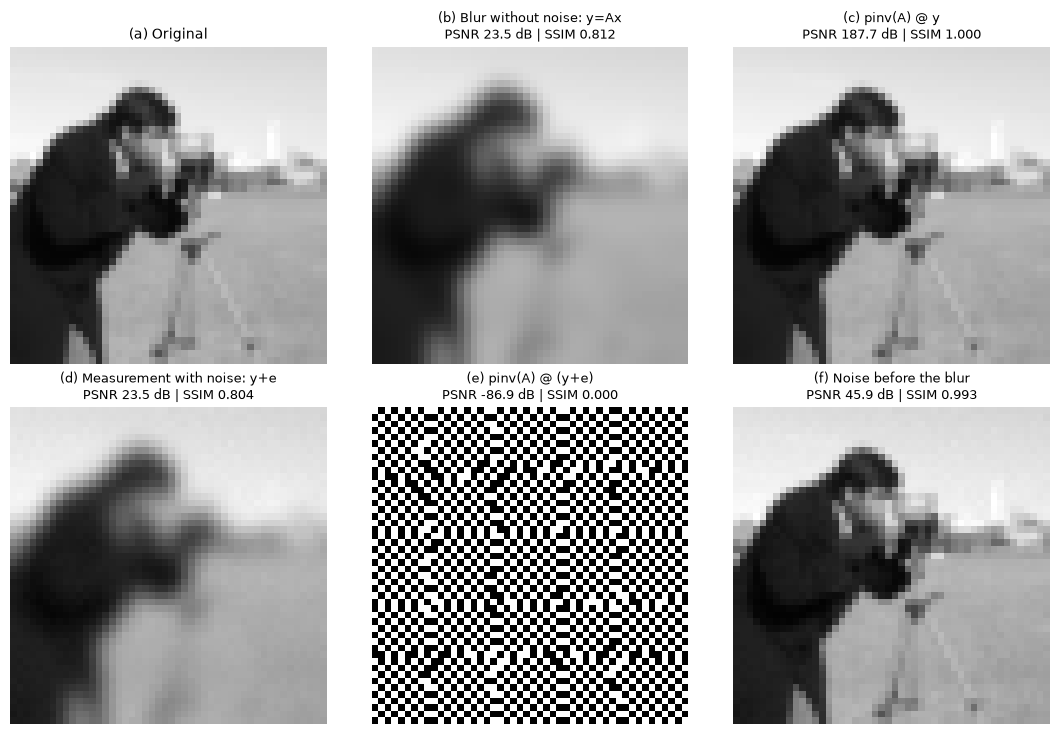
\includegraphics[width=\textwidth]{fig05_deconvolution.png}
\caption{Deconvolution experiment: (a) original image; (b) blurred data without noise; (c)
pseudoinverse of the clean data; (d) blurred data with noise added after the blur; (e)
pseudoinverse of the noisy data (noise amplified); (f) control with noise added before the blur.}
\label{fig:deconv}
\end{figure}

\subsection{Spectral analysis and noise sweep}

The singular values of $A$ decrease from approximately $1$ (the kernel has unit sum) to
$4\times10^{-9}$; their ratio is the condition number $2.44\times10^{8}$. As shown in
Figure~\ref{fig:spectrum} (left), $1394$ of the $2304$ singular values lie below the noise level
$\sigma_\eta=0.005$. In those directions the blur attenuates the signal more than the noise, so
the coefficients $u_i^\T y_\eta/\sigma_i$ are dominated by noise and the inversion is meaningless.

The right panel of Figure~\ref{fig:spectrum} repeats the experiment for nine noise levels between
$10^{-4}$ and $10^{-1}$ (five realizations each). On logarithmic axes, the error obtained when the
noise is added \emph{after} the blur grows with the data error but lies several orders of magnitude
above the no-amplification reference. When the noise is added \emph{before} the blur, the error
follows that reference, because the inversion cancels the blur and leaves the perturbation $e$
essentially unchanged.

\begin{figure}[htbp]
\centering
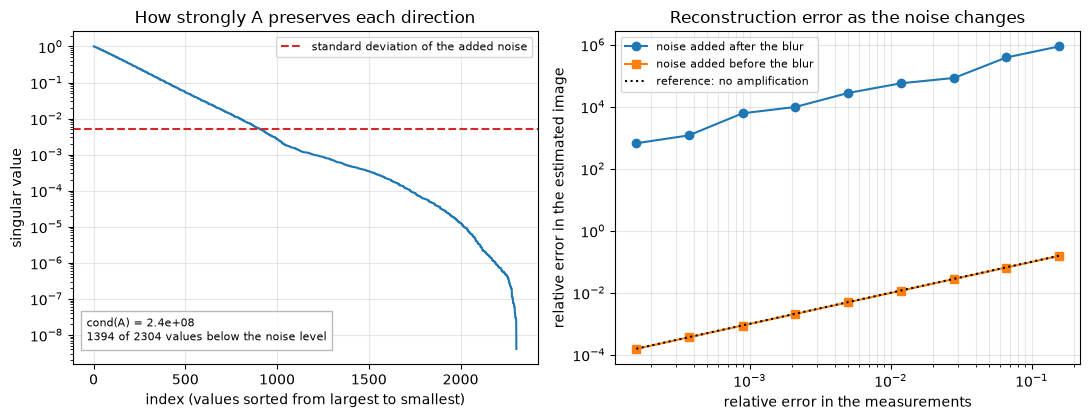
\includegraphics[width=\textwidth]{fig06_spectrum.png}
\caption{Left: singular values of $A$ in decreasing order; the dashed red line is the noise
standard deviation $\sigma_\eta=0.005$, and $1394$ of $2304$ values fall below it. Right:
relative error of the reconstructed image versus relative error of the measurements, for noise
added after the blur (circles) and before the blur (squares); the dotted line is the
no-amplification reference. Each point averages five realizations.}
\label{fig:spectrum}
\end{figure}

\paragraph{Why is direct inversion unstable?}
Solving $Ax=y$ amounts to dividing by the singular values $\sigma_i$ in \eqref{eq:errorprop}.
The blur strongly attenuates high-frequency directions, so their $\sigma_i$ are tiny. Any
measurement error has components in those directions, and dividing by $\sigma_i\ll1$ multiplies
them by factors up to $1/\sigma_{\min}\approx2.4\times10^{8}$. The result is the oscillatory,
checkerboard-like pattern of Figure~\ref{fig:deconv}e. Adding the noise before the blur is
harmless because then $e$ is part of the image being reconstructed, not an error in the data; the
pseudoinverse returns $x+e$. This confirms that the instability is caused by inverting a
severely ill-conditioned operator, not by the solver.

%=====================================================================
\section{Noisy deblurring with a sparse wavelet prior (ISTA)}\label{sec:ista}

\subsection{Regularized model and algorithm}

The reconstruction is now defined as
\begin{equation}
\hat{x}=\argmin_{x\in\R^N}\;
\underbrace{\frac12\|Ax-y_\eta\|_2^2}_{\text{data fidelity}}
+\lambda\underbrace{\|Wx\|_1}_{\text{sparsity prior}},
\qquad \lambda\ge0,
\label{eq:istaobj}
\end{equation}
where $W$ is an orthonormal wavelet transform (Daubechies \texttt{db2}, three levels,
periodization mode)~\cite{mallat2009}. The data term is smooth, with gradient
\begin{equation}
\nabla f(x)=A^\T(Ax-y_\eta),\qquad f(x)=\tfrac12\|Ax-y_\eta\|_2^2 ,
\label{eq:gradf}
\end{equation}
and the regularizer is convex but nonsmooth. ISTA alternates a gradient step on $f$ with the
proximal operator of $\lambda\|W\cdot\|_1$:
\begin{equation}
z_{k+1}=x_k-\eta\,A^\T(Ax_k-y_\eta),
\qquad
x_{k+1}=W^\T\operatorname{soft}\!\left(Wz_{k+1};\,\eta\lambda\right),
\label{eq:ista}
\end{equation}
starting from $x_0=0$, with the element-wise soft-thresholding operator
\begin{equation}
\operatorname{soft}(u;\alpha)=
\begin{cases}
u+\alpha, & u<-\alpha,\\
0, & |u|\le\alpha,\\
u-\alpha, & u>\alpha,
\end{cases}
\qquad
\operatorname{soft}(u;\alpha)=\operatorname{sign}(u)\max(|u|-\alpha,0).
\label{eq:soft}
\end{equation}

The proximal step is exact because $W$ is orthogonal. With $u=Wx$ and $c=Wz$, the problem
$\min_x\frac12\|x-z\|_2^2+\eta\lambda\|Wx\|_1$ becomes
$\min_u\frac12\|u-c\|_2^2+\eta\lambda\|u\|_1$, which separates into scalar problems whose solution
is $\operatorname{soft}(c;\eta\lambda)$. Hence
$\operatorname{prox}_{\eta\lambda\|W\cdot\|_1}(z)=W^\T\operatorname{soft}(Wz;\eta\lambda)$.

The step size is $\eta=1/L$ with $L=\|A^\T A\|_2=\sigma_{\max}^2$, estimated by $60$ power
iterations. The notebook obtains
\begin{equation}
L\approx0.9912,\qquad \eta=\frac{1}{L}\approx1.0089 .
\label{eq:Leta}
\end{equation}
The value $L\approx1$ is consistent with $\sigma_{\max}\approx1$ for a normalized blur kernel.
With $\eta\le1/L$, ISTA is guaranteed to decrease the objective~\eqref{eq:istaobj}
monotonically~\cite{beck2009}.

\paragraph{Sparsity of the image in the wavelet basis.}
The orthonormality of $W$ was verified numerically:
$\big|\|Wv\|_2-\|v\|_2\big|=7.1\times10^{-15}$ and
$\max|W^{-1}Wv-v|=1.6\times10^{-15}$. For the test image, $38$ of the $2304$ coefficients
($1.6\%$) carry $95\%$ of the energy and $163$ ($7.1\%$) carry $99\%$; moreover, $16.1\%$ of the
coefficients satisfy $|c|<10^{-3}$. This concentration, visible in Figure~\ref{fig:wavelet},
justifies the $\ell_1$ prior: keeping the few large coefficients preserves the structure, while
discarding the many small ones removes noise.

\begin{figure}[htbp]
\centering
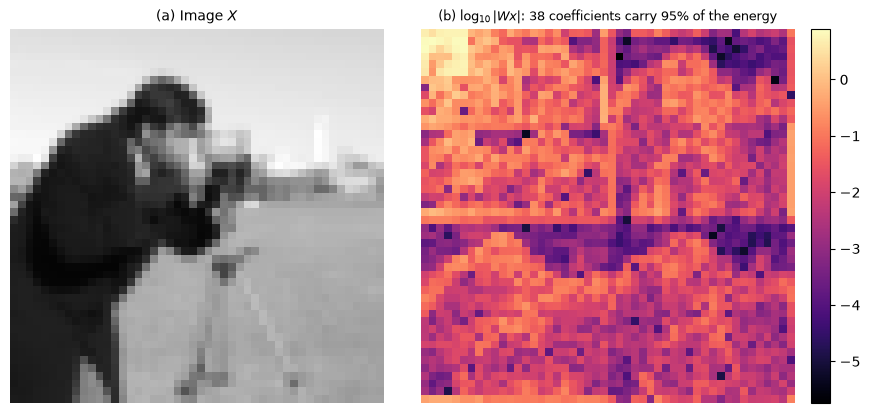
\includegraphics[width=0.9\textwidth]{fig07_wavelet.png}
\caption{(a) Test image $X$. (b) Magnitude of its wavelet coefficients on a logarithmic scale;
$38$ coefficients carry $95\%$ of the energy, which shows that the image is sparse in this basis.}
\label{fig:wavelet}
\end{figure}

\subsection{Choice of the regularization strength \texorpdfstring{$\lambda$}{lambda}}

Seven values of $\lambda$ were tested, each with $250$ ISTA iterations and $\eta$ from
\eqref{eq:Leta}. The results are given in Table~\ref{tab:lambda} and Figure~\ref{fig:ista}a.

\begin{table}[H]
\centering
\small
\begin{tabular}{ccc}
\toprule
$\lambda$ & PSNR (dB) & SSIM\\
\midrule
$1\times10^{-5}$ & $28.05$ & $0.874$\\
$2\times10^{-5}$ & $28.05$ & $0.877$\\
$3\times10^{-5}$ & $28.05$ & $0.879$\\
$5\times10^{-5}$ & $28.02$ & $0.883$\\
$1\times10^{-4}$ & $27.85$ & $0.886$\\
$3\times10^{-4}$ & $26.98$ & $0.877$\\
$1\times10^{-3}$ & $25.58$ & $0.853$\\
\bottomrule
\end{tabular}
\caption{Effect of $\lambda$ after $250$ ISTA iterations. The best PSNR is attained at
$\lambda=2\times10^{-5}$; the best SSIM at $\lambda=10^{-4}$.}
\label{tab:lambda}
\end{table}

PSNR is essentially flat for $\lambda\in[10^{-5},3\times10^{-5}]$ and then decreases, while SSIM
keeps improving up to $\lambda=10^{-4}$ before falling. The two metrics prefer slightly different
values because they measure different properties: PSNR is a pixelwise error, whereas SSIM rewards
structural similarity and tolerates stronger smoothing. A very small $\lambda$ leaves noise in the
reconstruction; a very large one ($10^{-3}$) over-smooths and erases texture. The value
$\lambda=2\times10^{-5}$ is selected because it maximizes PSNR.

\subsection{Iterations and early stopping}

Fixing $\lambda=2\times10^{-5}$ and running $1500$ iterations (metrics recorded every $10$), the
best PSNR is attained at iteration $260$:
\[
\text{PSNR}=28.05\ \text{dB},\qquad \text{SSIM}=0.876,
\]
while the last iterate at $1500$ iterations has PSNR $26.17$~dB and SSIM $0.752$. As shown in
Figure~\ref{fig:ista}b, the quality improves quickly and then degrades slowly. In contrast, the
objective \eqref{eq:istaobj} decreases monotonically (Figure~\ref{fig:ista}c), as guaranteed by
the theory.

This is the phenomenon of \emph{semi-convergence}: ISTA converges to the minimizer of the
regularized objective, but for a fixed, small $\lambda$ that minimizer still fits part of the
noise. Running more iterations therefore reduces the objective while moving away from the true
image. Early stopping acts as a second regularization mechanism. The best iteration was identified
using the known original image; in a real application it must be chosen by a data-driven rule
(e.g., the discrepancy principle or cross-validation).

\begin{figure}[htbp]
\centering
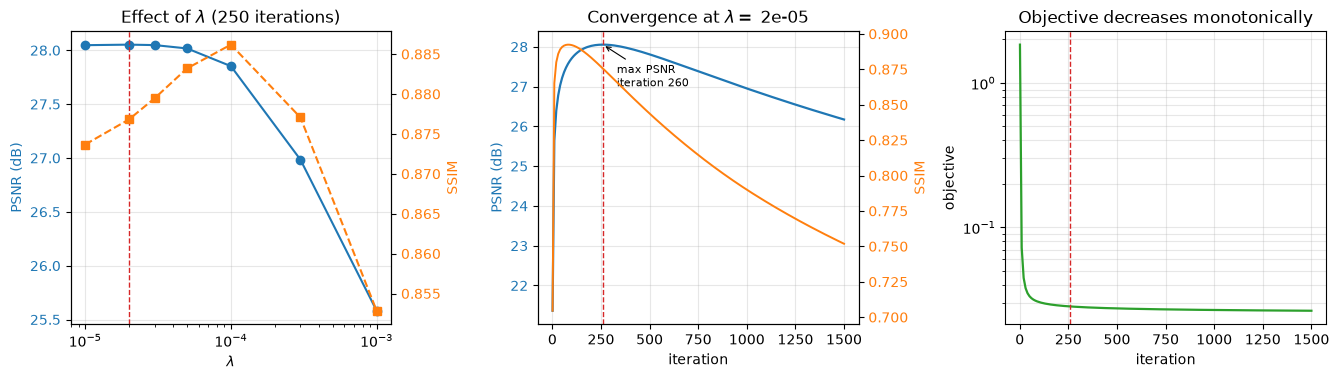
\includegraphics[width=\textwidth]{fig08_ista.png}
\caption{(a) PSNR and SSIM versus $\lambda$ after $250$ iterations; the red dashed line marks the
value selected by PSNR. (b) PSNR and SSIM during $1500$ iterations at $\lambda=2\times10^{-5}$;
the red line marks the best iteration ($260$). (c) The ISTA objective decreases monotonically
although the image quality eventually deteriorates.}
\label{fig:ista}
\end{figure}

\subsection{Comparison with direct inversion}

Table~\ref{tab:comparison} and Figure~\ref{fig:comparison} compare the blurred measurement, the
direct pseudoinverse of the noisy data, and ISTA after $10$ and $260$ iterations.

\begin{table}[H]
\centering
\small
\begin{tabular}{lcc}
\toprule
Method & PSNR (dB) & SSIM\\
\midrule
Blurred measurement            & $23.49$  & $0.812$\\
Direct inversion (pseudoinverse) & $-86.90$ & $0.000$\\
ISTA, $10$ iterations          & $25.64$  & $0.865$\\
ISTA, $260$ iterations         & $28.05$  & $0.876$\\
\bottomrule
\end{tabular}
\caption{Comparison between the blurred data, the direct inversion, and ISTA with
$\lambda=2\times10^{-5}$.}
\label{tab:comparison}
\end{table}

Already after $10$ iterations ISTA surpasses the blurred measurement, and at iteration $260$ it
gains $4.56$~dB over it (reaching $28.05$~dB), whereas the direct inversion gives $-86.90$~dB;
SSIM rises from $0.000$ to $0.876$. Visually, the oscillatory noise of the direct inversion disappears and the
main edges and textures are restored. The remaining error is mostly the high-frequency
information destroyed by the blur, which no inversion method can recover.

\begin{figure}[htbp]
\centering
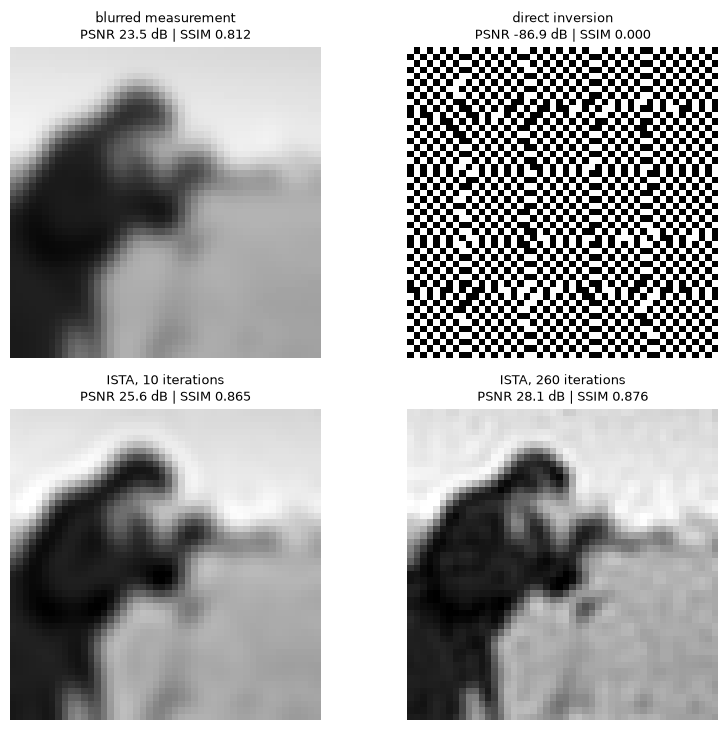
\includegraphics[width=0.72\textwidth]{fig09_comparison.png}
\caption{Top-left: blurred measurement. Top-right: direct inversion of the noisy data. Bottom-left:
ISTA after $10$ iterations. Bottom-right: ISTA at the best iteration ($260$). PSNR and SSIM are
shown above each panel.}
\label{fig:comparison}
\end{figure}

\subsection{Answers to the guiding questions}

\paragraph{What artifacts appear without a prior, and how does sparsity change them?}
The direct inversion produces a high-frequency checkerboard pattern caused by the amplified noise
in the directions where $\sigma_i\ll1$ (Figure~\ref{fig:deconv}e). The wavelet prior suppresses
these artifacts because the corresponding small wavelet coefficients are set to zero, while the
large coefficients associated with edges are retained. The result is a stable image with sharp
main structures instead of amplified noise.

\paragraph{Why does soft-thresholding reduce noise while preserving important coefficients?}
Natural images are sparse in the wavelet domain: a few large coefficients describe edges and
structure, and many small coefficients describe texture and noise. Additive noise spreads over all
coefficients, so the small ones are noise-dominated. Soft-thresholding maps every coefficient with
$|u|\le\eta\lambda$ to zero and shrinks the others by $\eta\lambda$. This removes the
noise-dominated coefficients and keeps the large, informative ones, at the cost of a small bias on
them.

\paragraph{What happens if $\lambda$ is too large or too small?}
If $\lambda$ is too small, the threshold $\eta\lambda$ removes almost nothing, the noise survives,
and the solution approaches the unstable least-squares inversion. The sweep shows the best PSNR at
$\lambda=2\times10^{-5}$. If $\lambda$ is too large, useful coefficients are also removed: at
$\lambda=10^{-3}$ the image is over-smoothed and both metrics fall ($25.58$~dB, SSIM $0.853$).
The useful range is roughly one decade, $10^{-5}$--$10^{-4}$.

\paragraph{How would a smoothness or total-variation prior change the result?}
A total-variation prior penalizes the $\ell_1$ norm of the image gradient instead of wavelet
coefficients, favoring piecewise-smooth images with sharp edges. Tikhonov smoothness, by contrast,
is quadratic and easy to implement but blurs edges. Both were implemented and compared in
Section~\ref{sec:priors}: with identical noisy data, TV reached $29.27$~dB and SSIM $0.925$,
Tikhonov $27.98$~dB and SSIM $0.863$, and the wavelet ISTA $28.05$~dB and SSIM $0.876$. TV
preserves the edges best, but it needs a primal-dual iteration (its proximal step has no closed
form) and can produce staircase artifacts on smooth gradients.

\paragraph{Does more iterations always mean a better image?}
No. The objective decreases monotonically, but the PSNR peaks at iteration $260$ and then declines;
at $1500$ iterations the PSNR has dropped to $26.17$~dB. Early stopping is therefore an additional
regularization parameter, as discussed in Section~\ref{sec:ista}.

%=====================================================================
\section{Alternative priors: Tikhonov smoothness and total variation}\label{sec:priors}

\subsection{Motivation and the two penalties}

The wavelet prior of Section~\ref{sec:ista} is only one member of a larger family of
regularizers. In general, any functional $R$ that measures how implausible an image is can be
used as a prior, and the workshop notes mention two classical alternatives to sparsity:
quadratic smoothness (Tikhonov) and piecewise smoothness (total variation). Both assume that
neighbouring pixels should be similar, so both can suppress the noise amplified by the inverse
of the blur, but they penalize jumps in very different ways.

Let $G\in\R^{2N\times N}$ be the discrete gradient: it stacks the horizontal and vertical
forward differences between neighbouring pixels, with Neumann (zero-difference) boundary
conditions. The two penalties are
\begin{equation}
R_{\text{Tik}}(x)=\frac12\|Gx\|_2^2
=\frac12\sum_{i=1}^{N}\left[(D_hx)_i^2+(D_vx)_i^2\right],
\qquad
R_{\text{TV}}(x)=\sum_{i=1}^{N}\sqrt{(D_hx)_i^2+(D_vx)_i^2}.
\label{eq:priors}
\end{equation}
Inside a flat region both penalties are zero. The difference is the growth for a jump of height
$h$: Tikhonov charges $\tfrac12 h^2$, which becomes very expensive for a strong edge, whereas TV
charges $|h|$, which grows only linearly. A quadratic penalty therefore prefers to spread an edge
over several pixels (it is blurred), while a linear penalty accepts a sharp edge at a bounded
cost. This is why TV is said to favour \emph{piecewise-smooth} images.

\subsection{Tikhonov smoothness: a quadratic prior}

The Tikhonov problem is
\begin{equation}
\hat{x}_\lambda=\argmin_{x\in\R^N}\;
\frac12\|Ax-y_\eta\|_2^2+\frac{\lambda}{2}\|Gx\|_2^2,
\qquad \lambda\ge0 .
\label{eq:tikobj}
\end{equation}
The objective is differentiable and strongly convex, so stationarity gives the linear system
\begin{equation}
\left(A^\T A+\lambda\,G^\T G\right)x=A^\T y_\eta .
\label{eq:tiknormal}
\end{equation}
Because $G^\T G\succeq0$ and $A$ is invertible, the matrix is positive definite and the solution
exists and is unique. With the SVD $A=U\Sigma V^\T$ and $G=I$, it has the closed form
\begin{equation}
\hat{x}_\lambda=\sum_{i=1}^{N}\frac{s_i^2}{s_i^2+\lambda}\,
\frac{u_i^\T y_\eta}{s_i}\,v_i .
\label{eq:tikfilter}
\end{equation}
The filter factor $s_i^2/(s_i^2+\lambda)$ is close to one for $s_i\gg\sqrt{\lambda}$ and close to
zero for $s_i\ll\sqrt{\lambda}$. Thus, instead of dividing by a tiny singular value and
amplifying the noise as the pseudoinverse does, Tikhonov \emph{damps} those directions. As
$\lambda\to0$ the pseudoinverse is recovered, and as $\lambda\to\infty$ the estimate tends to
zero. The price of the quadratic penalty is precisely the smoothing of the jumps discussed
above: the method is stable but blurs edges.

Equation~\eqref{eq:tiknormal} is solved with conjugate gradients, applying $A^\T A$ through its
SVD and $G^\T G$ as a sparse matrix; the normal matrix is never formed. The gradient operator has
$9024$ non-zero entries in a $4608\times2304$ matrix.

\subsection{Total variation and the Chambolle--Pock algorithm}

The total-variation problem replaces the squared gradient by its magnitude,
\begin{equation}
\hat{x}_\lambda=\argmin_{x\in\R^N}\;
\frac12\|Ax-y_\eta\|_2^2+\lambda\sum_{i=1}^{N}
\sqrt{(D_hx)_i^2+(D_vx)_i^2}.
\label{eq:tvobj}
\end{equation}
The penalty is an $\ell_1$ norm of the gradient: convex, but not differentiable where the
gradient vanishes, so there is no normal-equation solution. It is solved with the
Chambolle--Pock primal-dual algorithm~\cite{chambolle2011}. Introducing the dual variable $p$ for
the data term and $q=(q_h,q_v)$ for the gradient, one iteration reads
\begin{equation}
\begin{aligned}
p^{k+1}&=\frac{p^k+\sigma\left(A\bar{x}^k-y_\eta\right)}{1+\sigma},\\
q^{k+1}&=\operatorname{proj}_{\|\cdot\|_2\le\lambda}
\left(q^k+\sigma\,G\bar{x}^k\right),\\
x^{k+1}&=x^k-\tau\left(A^\T p^{k+1}+G^\T q^{k+1}\right),\\
\bar{x}^{k+1}&=2x^{k+1}-x^k .
\end{aligned}
\label{eq:cp}
\end{equation}
The projection onto the ball of radius $\lambda$ is applied pixel by pixel,
$q\leftarrow q/\max(1,\|q\|_2/\lambda)$. The iteration converges whenever
$\tau\sigma\|[A;G]\|_2^2<1$. Since $\|A\|_2^2=s_{\max}^2\approx0.9912$ and
$\|G\|_2^2\le8$, the choice $\tau=\sigma=0.99/\sqrt{s_{\max}^2+8}\approx0.33$ satisfies the
condition with a small safety margin.

\subsection{Choice of the regularization weight}

For a fair comparison, both priors use the same noisy measurement $y_\eta$ of
Section~\ref{sec:inv}. The Tikhonov problem was solved for six values of $\lambda$ and the TV
problem for five values, with $1500$ primal-dual iterations each. Tables~\ref{tab:tikhonov} and
\ref{tab:tv} list the results, and Figure~\ref{fig:priors} shows the two curves.

\begin{table}[H]
\centering
\small
\begin{tabular}{cccc}
\toprule
$\lambda$ & PSNR (dB) & SSIM & Note\\
\midrule
$1\times10^{-4}$ & $24.04$ & $0.644$ & too weak, noise remains\\
$3\times10^{-4}$ & $26.78$ & $0.772$ & \\
$1\times10^{-3}$ & $\mathbf{27.98}$ & $0.863$ & best PSNR\\
$3\times10^{-3}$ & $27.78$ & $0.892$ & \\
$1\times10^{-2}$ & $27.02$ & $\mathbf{0.893}$ & best SSIM\\
$3\times10^{-2}$ & $26.15$ & $0.880$ & over-smoothed\\
\bottomrule
\end{tabular}
\caption{Tikhonov smoothness: PSNR and SSIM versus $\lambda$ (conjugate gradients, tolerance
$10^{-8}$).}
\label{tab:tikhonov}
\end{table}

\begin{table}[H]
\centering
\small
\begin{tabular}{cccc}
\toprule
$\lambda$ & PSNR (dB) & SSIM & Note\\
\midrule
$1\times10^{-4}$ & $29.10$ & $0.916$ & \\
$2\times10^{-4}$ & $\mathbf{29.27}$ & $0.925$ & best PSNR\\
$3\times10^{-4}$ & $29.21$ & $\mathbf{0.926}$ & best SSIM\\
$5\times10^{-4}$ & $28.95$ & $0.924$ & \\
$1\times10^{-3}$ & $28.43$ & $0.916$ & over-smoothed\\
\bottomrule
\end{tabular}
\caption{Total variation: PSNR and SSIM versus $\lambda$ after $1500$ Chambolle--Pock iterations.}
\label{tab:tv}
\end{table}

Both curves have the expected U-shape: a small $\lambda$ leaves the amplified noise, and a large
one erases texture. The optimum is at $\lambda\approx10^{-3}$ for Tikhonov and at
$\lambda\approx2\times10^{-4}$ for TV. The two scales are not comparable, because the penalties
have different units and grow differently with the image size. Notice also that Tikhonov's PSNR
peaks earlier and then falls faster, while TV remains above $28.9$~dB over most of the tested
range: the edge-preserving penalty is more tolerant to the choice of $\lambda$.

\begin{figure}[htbp]
\centering
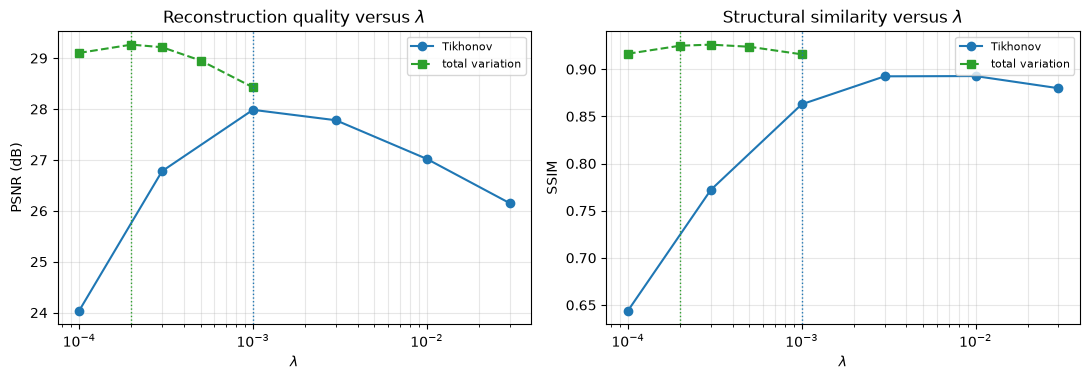
\includegraphics[width=\textwidth]{fig10_priors_sweep.png}
\caption{Tikhonov (circles) and total variation (squares) as a function of $\lambda$: PSNR (left)
and SSIM (right). The dotted vertical lines mark the value selected by PSNR for each prior.}
\label{fig:priors}
\end{figure}

\subsection{Comparison with the sparse wavelet prior}

Table~\ref{tab:priors} and Figure~\ref{fig:priorscomp} put the three priors side by side, always
using the same noisy data and the same metrics.

\begin{table}[H]
\centering
\small
\begin{tabular}{lcc}
\toprule
Method & PSNR (dB) & SSIM\\
\midrule
Blurred measurement                       & $23.49$  & $0.812$\\
Direct inversion (pseudoinverse)          & $-86.90$ & $0.000$\\
Tikhonov, $\lambda=10^{-3}$               & $27.98$  & $0.863$\\
Wavelet ISTA, $\lambda=2\times10^{-5}$     & $28.05$  & $0.876$\\
Total variation, $\lambda=2\times10^{-4}$  & $\mathbf{29.27}$ & $\mathbf{0.925}$\\
\bottomrule
\end{tabular}
\caption{Comparison of priors on the same noisy deblurring problem. ISTA uses its best iteration
($260$); TV uses $1500$ primal-dual iterations.}
\label{tab:priors}
\end{table}

\begin{figure}[H]
\centering
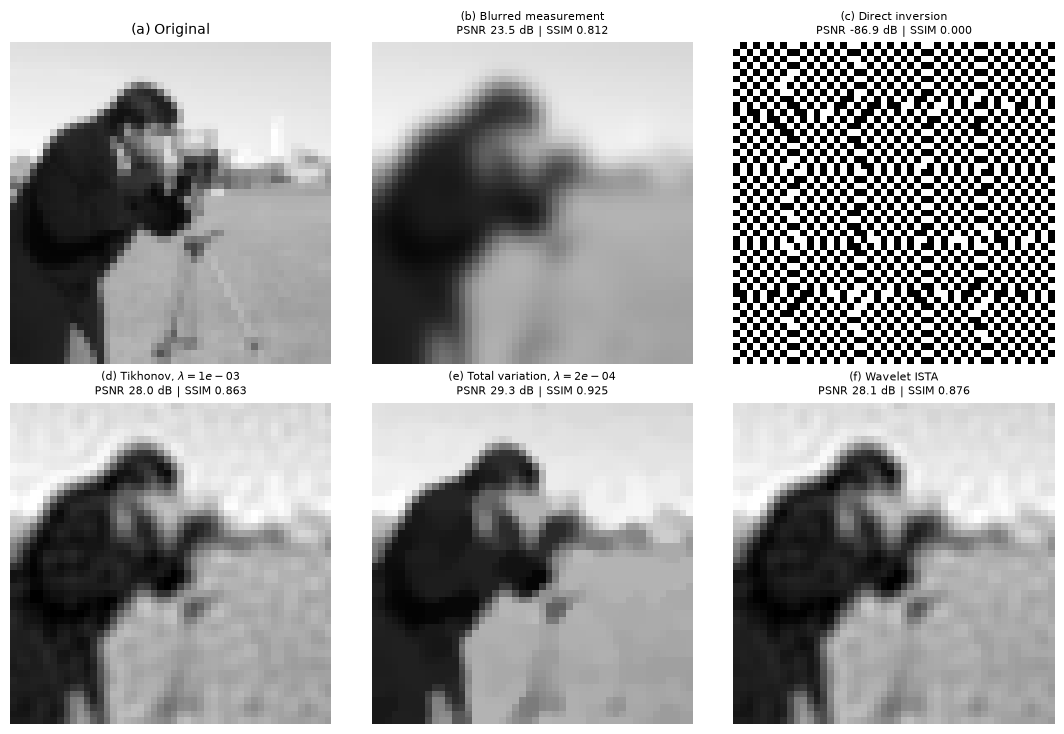
\includegraphics[width=\textwidth]{fig11_priors_comparison.png}
\caption{(a) Original image. (b) Blurred measurement. (c) Direct inversion. (d) Tikhonov at
$\lambda=10^{-3}$. (e) Total variation at $\lambda=2\times10^{-4}$. (f) Wavelet ISTA at its best
iteration. PSNR and SSIM are shown above each panel.}
\label{fig:priorscomp}
\end{figure}

TV gives the best result: $29.27$~dB and SSIM $0.925$, i.e.\ $5.78$~dB above the blurred
measurement, $1.21$~dB above the wavelet ISTA, and $1.28$~dB above Tikhonov. Visually, the
difference is explained by the shape of the penalty. Tikhonov removes the amplified noise of the
direct inversion but smooths the edges and leaves a mottled texture. TV removes the noise while
keeping the camera silhouette and the tripod legs sharp, because an edge costs only a fixed
amount and is not forced to spread. ISTA lies in between: the wavelet basis captures the
piecewise-smooth structure and some texture, but its thresholding is less effective at
reconstructing clean edges.

The cost of each method also differs. Tikhonov requires a single linear solve (conjugate
gradients, a few seconds). TV requires an iterative primal-dual method, and $1500$ iterations
were used here; its objective decreases monotonically and, unlike ISTA, the reconstruction does
not deteriorate appreciably if the iteration continues: at $4000$ iterations the PSNR is
$29.25$~dB, within $0.1$~dB of the value at $1500$. ISTA, by contrast, loses $1.9$~dB between
its best iteration ($260$) and $1500$ iterations, which is the semi-convergence discussed in
Section~\ref{sec:ista}.

\paragraph{Limitations.}
TV is not universally better. It can produce staircase plateaus on smooth gradients (visible as
flat patches in Figure~\ref{fig:priorscomp}e), and the ranking depends on the image: on a
texture-rich photograph the wavelet prior or a combination of priors may win. TV also requires
choosing $\lambda$ and the number of iterations, and each iteration is more expensive than an
ISTA step. The comparison nevertheless shows the main point: the choice of prior is a modelling
decision, and the shape of the penalty controls which structures survive the inversion.

%=====================================================================
\section{Conclusions}

\begin{enumerate}[leftmargin=1.6em,itemsep=2pt]
\item \textbf{1D optimization.} The quartic $f(x)=x^4-4x^2+x$ has three critical points:
$x\approx-1.4730$ (global minimum, $f\approx-5.4442$), $x\approx0.1260$ (local maximum), and
$x\approx1.3470$ (local minimum). Coercivity guarantees that the global minimum is attained.
\item \textbf{2D optimization.} The quadratic has the unique stationary point $(2/3,8/3)$; its
constant Hessian has eigenvalues $1$ and $3$, so it is positive definite and the point is the
global minimum, $f_{\min}=-28/3$.
\item \textbf{Least squares.} The normal equations give $A^\T A x=A^\T y$, and
$\nabla\|Ax-y\|^2=2A^\T(Ax-y)$. Numerically, \texttt{pinv} and \texttt{lstsq} agree to
$10^{-14}$. For $m>n$ the error is limited by noise ($4.47\times10^{-3}$); for $m<n$ the
pseudoinverse returns the minimum-norm solution, with zero residual but a large coefficient error
($0.893$).
\item \textbf{Deconvolution.} The blur matrix has $\kappa(A)=2.44\times10^{8}$. Inversion is exact
up to roundoff without noise (maximum error $1.73\times10^{-9}$) but amplifies noise added after
the blur by a factor $4.38\times10^{6}$, giving PSNR $-86.90$~dB. Noise added before the blur is not amplified:
the inversion returns the noisy image ($45.94$~dB). The difference is explained by
$\hat{x}-x=A^\dagger e$ and the division by the tiny singular values.
\item \textbf{Sparse reconstruction.} Only $38$ wavelet coefficients carry $95\%$ of the image
energy, which justifies an $\ell_1$ prior. With $\lambda=2\times10^{-5}$, ISTA reaches
$28.05$~dB and SSIM $0.876$ at iteration $260$, against $-86.90$~dB for direct inversion. The
objective decreases monotonically, but the PSNR peaks and then decreases, so early stopping is
also a regularization mechanism.
\item \textbf{Comparison of priors.} With the same noisy data, total variation attains
$29.27$~dB and SSIM $0.925$, the wavelet ISTA $28.05$~dB and $0.876$, and Tikhonov smoothness
$27.98$~dB and $0.863$; all three are far above the blurred measurement ($23.49$~dB) and the
direct inversion ($-86.90$~dB). The quadratic penalty of Tikhonov smooths edges, whereas the
linear growth of the TV penalty preserves them, which explains the $1.28$~dB gain. Tikhonov is
the cheapest method (one linear solve), TV the most expensive (a primal-dual iteration), and TV
can produce staircase artifacts on smooth gradients.
\item \textbf{Limits of the prior.} The priors stabilize the inversion and restore structure, but
they cannot recover the information dominated by noise: $1394$ of $2304$ singular directions are
already below the noise level. Better priors (learned denoisers, combinations of smoothness and
sparsity) or additional data are required to go further.
\end{enumerate}

\begin{thebibliography}{9}
\small
\bibitem{heckel2024}
R.~Heckel, \emph{Deep Learning for Computational Imaging}, lecture notes, 2024.

\bibitem{beck2009}
A.~Beck and M.~Teboulle, ``A fast iterative shrinkage-thresholding algorithm for linear inverse
problems,'' \emph{SIAM Journal on Imaging Sciences}, vol.~2, no.~1, pp.~183--202, 2009.

\bibitem{hansen2010}
P.~C. Hansen, \emph{Discrete Inverse Problems: Insight and Algorithms}. Philadelphia, PA: SIAM,
2010.

\bibitem{wang2004}
Z.~Wang, A.~C. Bovik, H.~R. Sheikh, and E.~P. Simoncelli, ``Image quality assessment: from error
visibility to structural similarity,'' \emph{IEEE Transactions on Image Processing}, vol.~13,
no.~4, pp.~600--612, 2004.

\bibitem{mallat2009}
S.~Mallat, \emph{A Wavelet Tour of Signal Processing: The Sparse Way}, 3rd ed. Burlington, MA:
Academic Press, 2009.

\bibitem{tikhonov1963}
A.~N. Tikhonov, ``Solution of incorrectly formulated problems and the regularization method,''
\emph{Soviet Mathematics Doklady}, vol.~4, pp.~1035--1038, 1963.

\bibitem{rof1992}
L.~I. Rudin, S.~Osher, and E.~Fatemi, ``Nonlinear total variation based noise removal
algorithms,'' \emph{Physica D}, vol.~60, no.~1--4, pp.~259--268, 1992.

\bibitem{chambolle2011}
A.~Chambolle and T.~Pock, ``A first-order primal-dual algorithm for convex problems with
applications to imaging,'' \emph{Journal of Mathematical Imaging and Vision}, vol.~40, no.~1,
pp.~120--145, 2011.
\end{thebibliography}

\end{document}
